%==============================================================================
% Artigo 1 - FGA0261 Inteligência Artificial II - 2026.2
% Formato: IEEE conference (classe IEEEtran, máximo 4 páginas)
% Entrega: 03/09/2026, pelo Microsoft Teams
%
% CONVENÇÃO DESTE ARQUIVO: uma frase por linha.
% Isso não muda o PDF (o LaTeX junta as linhas) e mantém o git diff legível
% quando as duas pessoas da dupla editam o mesmo parágrafo.
%
% Compilar: make no Linux; .\build.ps1 no Windows sem Perl/latexmk.
%==============================================================================
\documentclass[conference]{IEEEtran}

\usepackage[T1]{fontenc}
\usepackage[utf8]{inputenc}
% Para hifenização correta em português, descomente a linha abaixo.
% Exige o pacote texlive-langportuguese no Arch.
% \usepackage[brazil]{babel}

\usepackage{cite}
\usepackage{amsmath,amssymb,amsfonts}
\usepackage{graphicx}
\usepackage{booktabs}
\usepackage{url}

\graphicspath{{figs/}}
% Gerado automaticamente por python -m src.report.
% Fonte: os nove arquivos JSON canônicos em src/results/.
% Não editar manualmente.
\newcommand{\ResultRuns}{3}
\newcommand{\ResultDevice}{Tesla T4}
\newcommand{\ResultLogregFOne}{0{,}746 \pm 0{,}035}
\newcommand{\ResultLogregBalancedAccuracy}{0{,}760 \pm 0{,}028}
\newcommand{\ResultLogregAccuracy}{0{,}754 \pm 0{,}038}
\newcommand{\ResultLogregParametersTotal}{98\,312}
\newcommand{\ResultLogregParametersTrainable}{98\,312}
\newcommand{\ResultLogregTime}{247{,}2 \pm 91{,}4}
\newcommand{\ResultCnnFOne}{0{,}976 \pm 0{,}007}
\newcommand{\ResultCnnBalancedAccuracy}{0{,}975 \pm 0{,}007}
\newcommand{\ResultCnnAccuracy}{0{,}977 \pm 0{,}007}
\newcommand{\ResultCnnParametersTotal}{288\,488}
\newcommand{\ResultCnnParametersTrainable}{288\,488}
\newcommand{\ResultCnnTime}{301{,}9 \pm 63{,}6}
\newcommand{\ResultResnetFOne}{0{,}982 \pm 0{,}003}
\newcommand{\ResultResnetBalancedAccuracy}{0{,}981 \pm 0{,}003}
\newcommand{\ResultResnetAccuracy}{0{,}981 \pm 0{,}003}
\newcommand{\ResultResnetParametersTotal}{11\,180\,616}
\newcommand{\ResultResnetParametersTrainable}{11\,180\,616}
\newcommand{\ResultResnetTime}{254{,}7 \pm 91{,}0}
\newcommand{\ResultBestModel}{ResNet18}
\newcommand{\ResultBestFOne}{\ResultResnetFOne}


\begin{document}

\title{Comparação entre Regressão Logística, CNN e ResNet18 na Classificação de Células do BloodMNIST}

\author{
\IEEEauthorblockN{Gustavo Xavier Evangelista}
\IEEEauthorblockA{\textit{FGA0261 - Inteligência Artificial II} \\
\textit{Universidade de Brasília} \\
Brasília, Brasil \\
Matrícula: 241025247 \\
241025247@aluno.unb.br}
\and
\IEEEauthorblockN{Heitor Macêdo Ricardo}
\IEEEauthorblockA{\textit{FGA0261 - Inteligência Artificial II} \\
\textit{Universidade de Brasília} \\
Brasília, Brasil \\
Matrícula: 241039073 \\
241039073@aluno.unb.br}
}

\maketitle

\begin{abstract}
Classificar tipos celulares em imagens microscópicas auxilia a análise morfológica do sangue periférico, mas diferenças de frequência e semelhanças visuais entre classes dificultam comparações justas entre algoritmos.
Ainda há pouca evidência sobre o ganho progressivo de representações convolucionais e de transferência de aprendizado sobre uma linha de base linear sob um protocolo único.
Este trabalho compara regressão logística multinomial, uma rede neural convolucional compacta treinada do zero e uma ResNet18 pré-treinada no ImageNet-1K no BloodMNIST com resolução $64\times64$.
Os modelos foram avaliados nos splits oficiais, com o mesmo pré-processamento, três sementes e F1 macro como métrica principal; acurácia, acurácia balanceada, parâmetros e tempo de treinamento complementaram a análise.
A ResNet18 obteve F1 macro de $\ResultBestFOne$ no teste, ante $\ResultCnnFOne$ da CNN e $\ResultLogregFOne$ da regressão logística.
As duas arquiteturas convolucionais superaram amplamente a linha de base, enquanto a vantagem da ResNet18 sobre a CNN foi pequena e acompanhada de custo muito maior em parâmetros.
Os resultados sustentam o uso de representações espaciais neste benchmark, mas não validam diagnóstico clínico nem generalização para outros laboratórios.
\end{abstract}

\begin{IEEEkeywords}
BloodMNIST, classificação de células sanguíneas, redes neurais convolucionais, transferência de aprendizado, comparação de algoritmos
\end{IEEEkeywords}

%------------------------------------------------------------------------------
\section{Introdução}
\label{sec:introducao}
%------------------------------------------------------------------------------
% Alvo: ~0,6 página.
% Parágrafo 1: contexto e por que o problema importa.
% Parágrafo 2: o que já existe e o que falta (a lacuna).
% Parágrafo 3: frase explícita de contribuição -- "Este trabalho contribui com...".
% Parágrafo 4: mapa das seções.

A identificação dos tipos celulares em imagens microscópicas é uma tarefa básica da análise morfológica do sangue periférico e exige a distinção de células visualmente semelhantes por profissionais experientes \cite{acevedo2019recognition,acevedo2020dataset}.
O BloodMNIST reúne imagens de basófilos, eosinófilos, eritroblastos, granulócitos imaturos, linfócitos, monócitos, neutrófilos e plaquetas, totalizando oito classes com frequências distintas \cite{acevedo2020dataset,yang2023medmnist}.
Sua padronização em baixa resolução e em partições fixas permite comparar algoritmos de classificação sob condições controladas \cite{yang2023medmnist}.
Como o conjunto representa células normais isoladas e a resolução reduzida pode omitir detalhes relevantes, seu emprego neste estudo constitui um benchmark experimental, e não um sistema de apoio ao diagnóstico clínico \cite{acevedo2020dataset,yang2023medmnist}.

Redes neurais convolucionais (CNNs) e transferência de aprendizado já foram aplicadas às imagens que originaram o BloodMNIST, com ênfase em arquiteturas pré-treinadas e na acurácia global \cite{acevedo2019recognition,gavas2021deep}.
O estudo de referência do MedMNIST também avalia redes residuais e métodos automatizados, porém não isola, em um único protocolo com múltiplas sementes, o ganho progressivo de uma CNN compacta e de uma rede pré-treinada sobre um classificador linear em F1 macro \cite{yang2023medmnist}.
Permanece, portanto, a necessidade de uma comparação controlada das três famílias que considere o desbalanceamento entre os tipos celulares e também seus custos computacionais \cite{acevedo2020dataset,yang2023medmnist}.
Diante dessa lacuna, formula-se a pergunta de pesquisa: em classificação multiclasse de tipos celulares no BloodMNIST, em que medida uma CNN compacta treinada do zero e uma ResNet18 pré-treinada no ImageNet-1K superam uma regressão logística em F1 macro, sob o mesmo protocolo experimental?

Este trabalho contribui com: (i) uma comparação controlada entre regressão logística multinomial, CNN compacta treinada do zero e ResNet18 pré-treinada no ImageNet-1K; (ii) uma análise conjunta de F1 macro, acurácia balanceada, tempo de treino e número de parâmetros em três sementes aleatórias.

O restante do artigo está organizado da seguinte forma.
A Seção~\ref{sec:trabalhos} discute os trabalhos relacionados.
A Seção~\ref{sec:metodologia} descreve a metodologia adotada.
A Seção~\ref{sec:resultados} apresenta os resultados.
A Seção~\ref{sec:discussao} discute os achados e as limitações, e a Seção~\ref{sec:conclusao} conclui o trabalho.

%------------------------------------------------------------------------------
\section{Trabalhos Relacionados}
\label{sec:trabalhos}
%------------------------------------------------------------------------------
% Alvo: ~0,5 página, 5 a 8 referências.
% Agrupe por abordagem, não faça uma lista de resumos individuais.
% Feche a seção dizendo o que este trabalho faz de diferente.

Classificadores lineares, como a regressão logística multinomial, estimam fronteiras de decisão diretamente sobre atributos fixos e oferecem uma referência simples para quantificar o valor acrescentado por representações não lineares \cite{bohning1992multinomial,goodfellow2016deep}.
Quando recebem pixels vetorizados, entretanto, esses classificadores não incorporam explicitamente a localidade nem o compartilhamento de parâmetros característicos das imagens \cite{goodfellow2016deep,lecun2015deep}.

As CNNs exploram esses dois vieses por meio de filtros convolucionais e constroem representações espaciais hierárquicas durante o treinamento \cite{lecun2015deep}.
Uma CNN compacta inicializada aleatoriamente constitui, assim, um nível intermediário de comparação: aprende atributos específicos do BloodMNIST sem recorrer a dados externos, mas dispõe de menor capacidade que arquiteturas profundas \cite{goodfellow2016deep,lecun2015deep}.

Na transferência de aprendizado, filtros aprendidos em uma tarefa de origem podem ser reutilizados, embora sua generalidade tenda a diminuir nas camadas superiores \cite{yosinski2014transferable}.
As redes residuais facilitam a otimização de arquiteturas profundas mediante conexões de atalho, propriedade que fundamenta o uso da ResNet18 como modelo transferido \cite{he2016deep}.
No conjunto de células sanguíneas que deu origem ao BloodMNIST, foram avaliadas redes VGG-16 e InceptionV3 como extratoras de atributos e em ajuste fino, enquanto outro estudo comparou 27 CNNs pré-treinadas no ImageNet \cite{acevedo2019recognition,gavas2021deep}.
O benchmark MedMNIST padronizou partições e incluiu ResNet18 e ResNet50 entre suas referências, favorecendo comparações reprodutíveis entre métodos \cite{yang2023medmnist}.

Diferentemente desses estudos, este artigo compara um classificador linear, uma CNN compacta treinada do zero e uma ResNet18 com ajuste fino integral nas mesmas partições oficiais e com imagens de resolução $64\times64$, usando três sementes e F1 macro como critério principal.

%------------------------------------------------------------------------------
\section{Metodologia}
\label{sec:metodologia}
%------------------------------------------------------------------------------
% Alvo: ~1,0 página. É a seção mais densa e um dos critérios de correção.
% Regra: outra pessoa tem que conseguir reproduzir o experimento lendo só isto.

\subsection{Conjunto de Dados}
Foi utilizado o BloodMNIST na resolução $64\times64$, subconjunto do MedMNIST+ derivado de imagens microscópicas de células individuais do sangue periférico e distribuído como um conjunto público para classificação multiclasse \cite{acevedo2020dataset,yang2024medmnistdata}.
O artefato contém 17\,092 imagens em três canais de cor vermelho, verde e azul (RGB), rotuladas em oito classes: 1\,218 basófilos, 3\,117 eosinófilos, 1\,551 eritroblastos, 2\,895 granulócitos imaturos, 1\,214 linfócitos, 1\,420 monócitos, 3\,329 neutrófilos e 2\,348 plaquetas.
As frequências variam de 7,10\% para linfócitos a 19,48\% para neutrófilos, o que caracteriza desbalanceamento moderado entre as classes.
Os dados foram obtidos pela interface de programação de aplicações (API) do MedMNIST, versão 3.0.2, com o identificador \texttt{bloodmnist}, resolução 64 e download automático a partir do registro oficial no Zenodo indicado em \cite{yang2024medmnistdata}, sob a licença Creative Commons Attribution 4.0 (CC BY 4.0).

\subsection{Pré-processamento}
Foram usadas as imagens previamente recortadas ao centro e redimensionadas para $64\times64$ pelo MedMNIST+.
Após a conversão dos valores inteiros para tensores no intervalo $[0,1]$, cada canal foi normalizado pelas médias $(0{,}7961, 0{,}6596, 0{,}6963)$ e pelos desvios padrão $(0{,}2233, 0{,}2546, 0{,}0947)$, calculados exclusivamente sobre o conjunto de treino para evitar vazamento de informação.
Durante o treino, aplicaram-se independentemente espelhamentos horizontal e vertical, ambos com probabilidade 0,5, e rotação aleatória de até $15^\circ$ em cada direção.
Na validação e no teste não houve aumento de dados, mas foi mantida a normalização estimada no treino.
Não foi necessária imputação, pois o artefato utilizado não contém imagens ou rótulos ausentes.

\subsection{Protocolo Experimental}
Foram preservados os splits oficiais e fixos do BloodMNIST, com 11\,959 imagens para treino, 1\,712 para validação e 3\,421 para teste, correspondentes aproximadamente à razão 70:10:20.
As proporções das oito classes são praticamente idênticas nos três splits, e nenhuma redivisão ou amostragem estratificada adicional foi realizada.
Cada modelo foi treinado com as sementes 42, 1337 e 2026, totalizando nove execuções independentes; as sementes alteraram a inicialização, a ordem dos lotes e as transformações aleatórias, mas não a composição dos splits, e o modo determinístico do backend cuDNN foi ativado.
Todos os modelos foram avaliados sob o mesmo protocolo, com as mesmas imagens, pré-processamento, tamanho de lote, limite de épocas e regra de seleção; as variações específicas de modelo restringiram-se à arquitetura, à inicialização e às taxas de aprendizado declaradas a seguir.
O desenvolvimento e os testes curtos ocorreram localmente, enquanto as nove execuções finais foram realizadas no mesmo ambiente do Google Colab, e o conjunto de teste foi consultado somente após a seleção da melhor época pela validação.

\subsection{Modelos e Hiperparâmetros}
Foram comparadas três famílias de classificadores com complexidade crescente.
A regressão logística multinomial lineariza os $3\times64\times64$ valores da imagem e os conecta diretamente às oito saídas, totalizando 98\,312 parâmetros treináveis.
A rede neural convolucional (CNN) compacta foi treinada do zero e contém três blocos com 32, 64 e 128 canais; cada bloco aplica duas convoluções $3\times3$ com preenchimento unitário, normalização em lote e unidade linear retificada (ReLU), seguidas por subamostragem pelo máximo (max-pooling) $2\times2$.
Após os blocos, foram usados pooling médio adaptativo, dropout de 0,3 e uma camada linear de 128 para oito unidades, em um total de 288\,488 parâmetros treináveis.
A ResNet18 \cite{he2016deep} foi inicializada com os pesos ImageNet-1K \cite{deng2009imagenet} identificados por \texttt{IMAGENET1K\_V1}, teve sua camada final substituída por uma projeção de 512 para oito classes e foi integralmente ajustada, com 11\,180\,616 parâmetros treináveis.
Os três modelos foram otimizados com AdamW, decaimento de pesos de $10^{-4}$ e entropia cruzada multiclasse sem ponderação por classe ou reamostragem.
A taxa de aprendizado foi de $10^{-3}$ para a regressão logística e a CNN; na ResNet18, adotaram-se $10^{-4}$ no corpo da rede e $10^{-3}$ na camada final.
O tamanho de lote foi 64 e o limite foi de 30 épocas, com parada antecipada após cinco épocas consecutivas sem melhora superior a $10^{-4}$ no F1 macro de validação; o estado de maior F1 macro foi restaurado antes do teste.
A implementação utilizou Python 3.13.15, PyTorch 2.11.0+cu128 e torchvision 0.26.0+cu128, e as execuções canônicas foram feitas em uma unidade de processamento gráfico (GPU) NVIDIA Tesla T4 a partir do commit \texttt{7ac7cc5}.

\begin{table*}[t]
\caption{Desempenho no conjunto de teste, contagem de parâmetros e tempo de treinamento no mesmo ambiente Google Colab com GPU \ResultDevice{}; métricas e tempo são apresentados como média $\pm$ desvio padrão de \ResultRuns{} sementes, permitindo comparar qualidade preditiva, estabilidade e custo computacional.}
\label{tab:resultados}
\centering
\begin{tabular}{lcccccc}
\toprule
Modelo & F1 macro & Acurácia balanceada & Acurácia & \multicolumn{2}{c}{Parâmetros} & Tempo (s) \\
\cmidrule(lr){5-6}
& & & & Totais & Treináveis & \\
\midrule
Regressão logística & $\ResultLogregFOne$ & $\ResultLogregBalancedAccuracy$ & $\ResultLogregAccuracy$ & $\ResultLogregParametersTotal$ & $\ResultLogregParametersTrainable$ & $\ResultLogregTime$ \\
CNN compacta & $\ResultCnnFOne$ & $\ResultCnnBalancedAccuracy$ & $\ResultCnnAccuracy$ & $\ResultCnnParametersTotal$ & $\ResultCnnParametersTrainable$ & $\ResultCnnTime$ \\
ResNet18 & $\mathbf{\ResultResnetFOne}$ & $\ResultResnetBalancedAccuracy$ & $\ResultResnetAccuracy$ & $\ResultResnetParametersTotal$ & $\ResultResnetParametersTrainable$ & $\ResultResnetTime$ \\
\bottomrule
\end{tabular}
\end{table*}

\subsection{Métricas}
A métrica principal foi o F1 macro, calculado pela média não ponderada do F1 das oito classes, porque a variação de frequência entre tipos celulares faria a acurácia favorecer as classes mais numerosas \cite{sokolova2009systematic}.
A acurácia foi mantida como medida da proporção global de acertos, e a acurácia balanceada, definida pela média da sensibilidade (recall) por classe, foi usada para verificar o desempenho sem ponderação pela prevalência.
A matriz de confusão permitiu localizar os pares de classes responsáveis pelos erros.
O tempo de treino e os números de parâmetros totais e treináveis foram registrados para relacionar o ganho preditivo ao custo computacional de cada arquitetura.
Para cada modelo, as métricas de teste foram resumidas pela média e pelo desvio padrão amostral das três sementes.
% Justificar a métrica é um critério de correção explícito do professor.
% Acurácia em base desbalanceada é o erro mais comum: use F1, AUC-ROC ou
% acurácia balanceada e diga por quê.

%------------------------------------------------------------------------------
\section{Resultados}
\label{sec:resultados}
%------------------------------------------------------------------------------
% Alvo: ~0,8 página. Uma tabela principal e uma figura que responda a uma pergunta.
% Não escreva prosa descrevendo a tabela: comente apenas o que ela não mostra.

Sob o protocolo comum, a Tabela~\ref{tab:resultados} mostra que os dois modelos convolucionais superaram a regressão logística em F1 macro e que a ResNet18 alcançou a maior média.
A tabela não identifica quais pares de tipos celulares concentram os erros nem se o desempenho agregado oculta dificuldades recorrentes em classes específicas.

\begin{figure}[htbp]
\centering
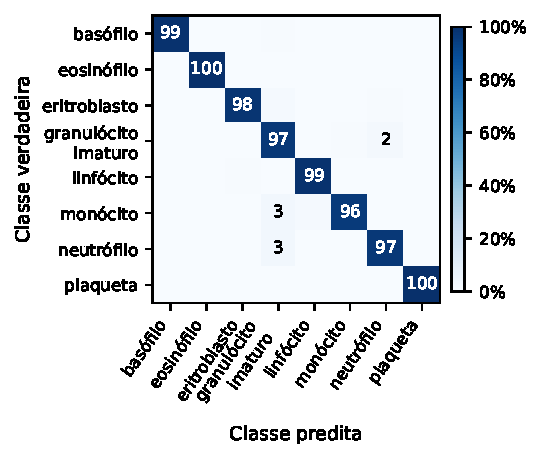
\includegraphics[width=\columnwidth]{confusao-melhor-modelo.pdf}
\caption{Matriz de confusão da \ResultBestModel{}, agregada nas \ResultRuns{} sementes e normalizada por classe verdadeira; essa normalização torna visíveis os tipos celulares que concentram erros e que as médias globais não distinguem.}
\label{fig:confusao-melhor-modelo}
\end{figure}

A Figura~\ref{fig:confusao-melhor-modelo} complementa a tabela ao localizar as confusões do melhor modelo entre granulócitos imaturos e neutrófilos.

%------------------------------------------------------------------------------
\section{Discussão e Limitações}
\label{sec:discussao}
Os ganhos de 0,230 e 0,236 em F1 macro da CNN e da ResNet18 sobre a regressão logística, respectivamente, indicam que explorar a estrutura espacial das imagens foi mais importante que aplicar um classificador diretamente aos pixels vetorizados.
A maior média da ResNet18 é compatível com sua maior capacidade e com a reutilização de filtros visuais aprendidos no ImageNet-1K, seguida pelo ajuste de toda a rede ao domínio alvo \cite{yosinski2014transferable,he2016deep}; essa associação, entretanto, não estabelece isoladamente uma relação causal.

Na matriz agregada da ResNet18, as confusões mais frequentes ocorreram entre granulócitos imaturos e neutrófilos: 39 de 1\,737 granulócitos imaturos foram classificados como neutrófilos (2,2\%), enquanto 59 de 1\,998 neutrófilos receberam o rótulo de granulócito imaturo (3,0\%).
Também houve 24 de 852 monócitos classificados como granulócitos imaturos (2,8\%).
Esses erros são coerentes com uma tarefa que depende de diferenças morfológicas finas entre células visualmente relacionadas, justamente o tipo de informação que pode ser reduzido na resolução adotada \cite{acevedo2020dataset}.
A diferença de 0,006 entre a ResNet18 ($0{,}982\pm0{,}003$) e a CNN ($0{,}976\pm0{,}007$) foi menor que o desvio padrão da CNN e da mesma ordem da variação entre sementes; com apenas três execuções e sem teste de hipótese, não se pode afirmar superioridade estatística da ResNet18.

Quanto ao custo, a CNN obteve grande ganho sobre a regressão logística com 288\,488 parâmetros e tempo médio de 301,9 s, ante 98\,312 parâmetros e 247,2 s da linha de base.
A ResNet18 elevou o F1 macro em apenas 0,006 sobre a CNN, mas utilizou 11\,180\,616 parâmetros, aproximadamente 38,8 vezes mais; seus 254,7 s médios não permitem concluir que tenha sido mais rápida, pois os desvios dos tempos foram elevados e houve parada antecipada em épocas diferentes.
Assim, a CNN oferece o compromisso mais econômico, enquanto a ResNet18 fornece a maior média quando memória e tamanho do modelo não são restrições.

Há três limitações principais.
Primeiro, as imagens reduzidas a $64\times64$, as frequências diferentes entre as oito classes e a origem microscópica restrita do BloodMNIST limitam a informação visual e a diversidade dos dados.
Segundo, foram usadas somente três sementes, sem teste estatístico e com busca limitada de hiperparâmetros para os três modelos.
Terceiro, este benchmark de células normais isoladas não valida diagnóstico clínico nem demonstra generalização para outros laboratórios, equipamentos, populações ou resoluções.

%------------------------------------------------------------------------------
\section{Conclusão}
\label{sec:conclusao}
Sob o mesmo protocolo experimental, a CNN compacta e a ResNet18 superaram a regressão logística em 0,230 e 0,236 de F1 macro, respectivamente, confirmando o benefício das representações convolucionais para o BloodMNIST.
A ResNet18 apresentou a maior média, de $\ResultBestFOne$, mas seu ganho de 0,006 sobre a CNN foi pequeno diante da variação entre sementes e exigiu aproximadamente 38,8 vezes mais parâmetros.
Conclui-se que a CNN compacta oferece o melhor compromisso entre desempenho e complexidade neste benchmark, enquanto a ResNet18 prioriza a maior média preditiva.
Trabalhos futuros devem ampliar o número de sementes, aplicar testes estatísticos, explorar hiperparâmetros de forma sistemática e avaliar imagens externas obtidas em outros laboratórios e resoluções.

%------------------------------------------------------------------------------
% REFERÊNCIAS - 10 a 15 itens, incluindo obrigatoriamente o conjunto de dados.
%------------------------------------------------------------------------------
\IEEEtriggeratref{7}
\bibliographystyle{IEEEtran}
\bibliography{refs}

\end{document}
